\documentclass[12pt,a4paper]{article}
\usepackage[utf8]{vietnam}
\usepackage{amsmath,amssymb}
\usepackage{tikz,pgfplots,tkz-tab}
\usepackage{tcolorbox}
\usepackage{multicol,longtable,booktabs,multirow}
\usepackage[version=4]{mhchem}
\usepackage{siunitx}
\usetikzlibrary{calc,patterns,arrows.meta,decorations.pathmorphing}
\pgfplotsset{compat=1.18}
\newcommand{\bonpa}[4]{\par\noindent\textbf{A.} #1 \quad \textbf{B.} #2 \quad \textbf{C.} #3 \quad \textbf{D.} #4\par}
\newcommand{\dinhnghia}[1]{\textbf{Định nghĩa.} #1}
\begin{document}

\section*{Bộ kiểm thử cấu trúc lạ}

\textbf{Câu 1.} Công thức quen: $\displaystyle\int_0^1 \frac{x^2}{\sqrt{1+x^3}}\,dx$ và $\ce{2H2 + O2 -> 2H2O}$, đo \SI{9.8}{m/s^2}.
\bonpa{$1$.}{$2$.}{$3$.}{$4$.}

\textbf{Câu 2.} Bảng biến thiên tkz-tab:
\begin{center}
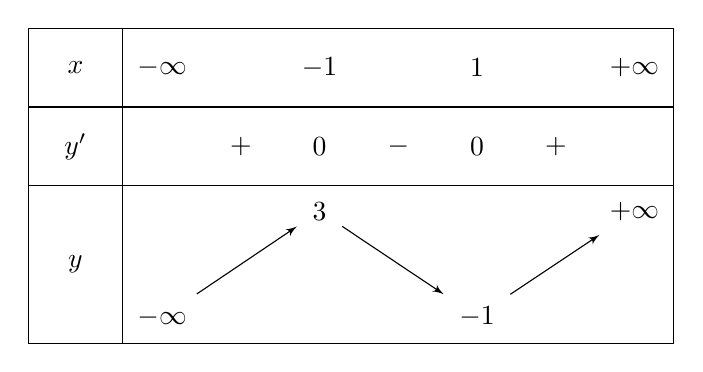
\begin{tikzpicture}
\tkzTabInit[lgt=1.2,espcl=2]{$x$/1,$y'$/1,$y$/2}{$-\infty$,$-1$,$1$,$+\infty$}
\tkzTabLine{,+,0,-,0,+,}
\tkzTabVar{-/$-\infty$,+/$3$,-/$-1$,+/$+\infty$}
\end{tikzpicture}
\end{center}

\textbf{Câu 3.} Đồ thị pgfplots:
\begin{center}
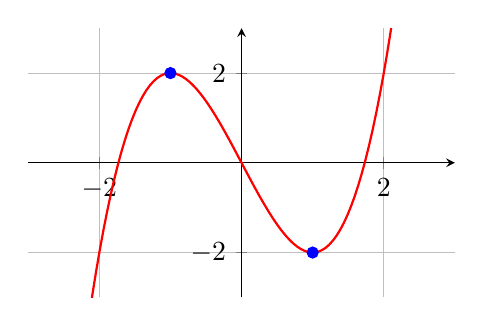
\begin{tikzpicture}
\begin{axis}[axis lines=middle,width=7cm,height=5cm,xmin=-3,xmax=3,ymin=-3,ymax=3,grid=both]
\addplot[thick,red,domain=-2.5:2.5,samples=100]{x^3-3*x};
\addplot[only marks,blue] coordinates {(-1,2) (1,-2)};
\end{axis}
\end{tikzpicture}
\end{center}

\textbf{Câu 4.} Khung tcolorbox bo góc có bóng:
\begin{tcolorbox}[colback=yellow!10,colframe=red!60!black,title=Ghi nhớ quan trọng]
Với mọi $a,b>0$ ta có $\dfrac{a+b}{2}\ge\sqrt{ab}$.
\end{tcolorbox}

\textbf{Câu 5.} Hình TikZ vẽ tay có hoa văn và mũi tên lạ:
\begin{center}
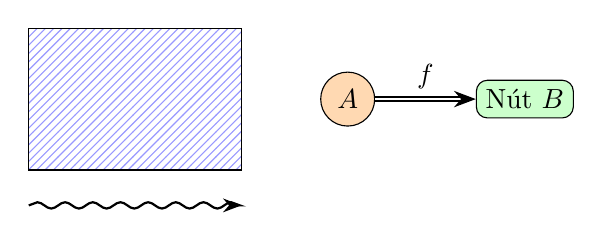
\begin{tikzpicture}[scale=0.9,>=Stealth]
\draw[pattern=north east lines,pattern color=blue!40] (0,0) rectangle (3,2);
\draw[->,thick,decorate,decoration={snake,amplitude=.4mm}] (0,-0.5) -- (3,-0.5);
\node[draw,circle,fill=orange!30] (A) at (4.5,1) {$A$};
\node[draw,rounded corners,fill=green!20] (B) at (7,1) {Nút $B$};
\draw[->,double,thick] (A) -- (B) node[midway,above]{$f$};
\end{tikzpicture}
\end{center}

\textbf{Câu 6.} Môi trường HOÀN TOÀN LẠ chưa ai khai báo:
\begin{bangxetdauthan}[kieu=dep]
\hang{$x$}{$-\infty$}{$0$}{$+\infty$}
\hang{$f'$}{$+$}{$0$}{$-$}
\end{bangxetdauthan}

\textbf{Câu 7.} Lệnh lạ chưa ai khai báo: \veanhlaso[cao=3cm]{parabol}{y=x^2} và \tomauvung{xanh}.

\textbf{Câu 8.} Gói chắc chắn KHÔNG có trên máy:
\begin{center}
\begin{khongtontai}
\vecaigiday{1}{2}
\end{khongtontai}
\end{center}

\textbf{Câu 9.} Bảng dài nhiều cột:
\begin{center}
\begin{tabular}{|c|c|c|c|}
\hline
\multirow{2}{*}{Nhóm} & \multicolumn{3}{c|}{Tần số} \\ \cline{2-4}
 & $n_1$ & $n_2$ & $n_3$ \\ \hline
$[0;5)$ & 3 & 5 & 7 \\ \hline
\end{tabular}
\end{center}

\dinhnghia{Hàm số liên tục trên đoạn $[a;b]$ nếu \ldots}

\end{document}
